\section{System model and problem formulation}
\label{sec:system}

\subsection{Near-RT RIC and conflict mitigation}
\label{sec:setting_ric}

The system consists of a near-RT RIC that hosts xApps and controls a set of cells (Figure~\ref{fig:system}). Each xApp
reads cell reports and requests changes to its parameter families, each of which has one writer. An O-RAN-style
conflict-mitigation interface~\cite{ORANConflictMit,ORANRICARCH} accepts or rejects each request; we call its rule the
referee. Rejected requests are not applied and may be proposed again. Per-cell KPIs summarise network state, including
protected-slice and service violations, energy, radio-link failures (RLFs) and served load; violations count violated
UE-seconds. The own, neighbour and far relations distinguish the request's cell, its neighbours and all remaining
cells.

\begin{figure}[tbp]
\centering
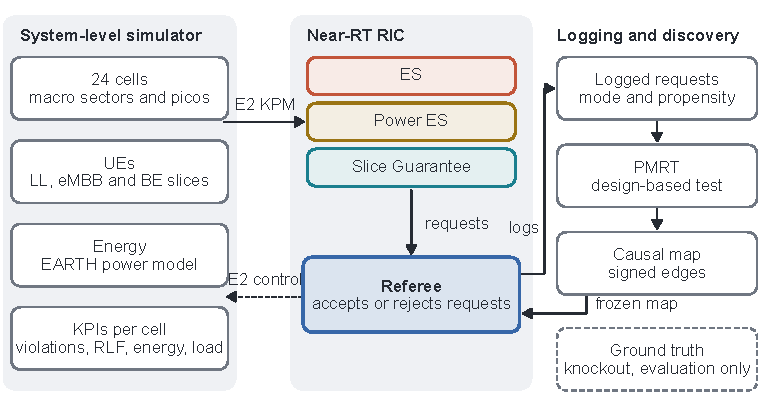
\includegraphics[width=\textwidth]{figures/fig_system.pdf}
\caption{System model.}
\label{fig:system}
\end{figure}

\subsection{Decision units and logging}
\label{sec:units}\claim{DEF-SYS-UNIT}\claim{DEF-SYS-LOG}

The referee decides per decision unit rather than per request. A unit $u$, identified by a cell, xApp and opening
time, opens at the pair's first request while none of its units is active. Its accept-or-reject mode $W_u$ is drawn
once and held for $t_{\mathrm{hold}} = 60$~s; all requests of the pair during the hold inherit it. The RIC records the
mode and its acceptance propensity $\pi_u$. Each unit also carries observation-only context from its opening request,
recent cell reports and applied configuration, including neighbour aggregates. Discovery uses only these logs and the
per-cell KPI series.

Three logging policies are considered. The uniform-randomised policy accepts each unit independently with probability
0.5. Under the state-dependent incumbent policy, the propensity, within $[0.15, 0.85]$, depends on the request class
and prior cell state: physical resource block (PRB) utilisation for energy-saving requests and the share of protected
user equipments (UEs) below their throughput floor for protected-share requests. Placebo logs draw and record modes
in the same way but apply every request.

\subsection{Problem formulation}
\label{sec:estimand}\claim{DEF-SYS-HYP}\claim{DEF-EST-H0}\claim{DEF-SYS-MITIG}

A hypothesis $(f, r, k)$ concerns a parameter family $f$, a relation $r$ and a KPI $k$; in the scenario of
Section~\ref{sec:design}, four families, three relations and five KPIs give $m = 60$ hypotheses. Because the referee
randomises the mode of a unit rather than a parameter value, each hypothesis concerns a mode contrast held for
$t_{\mathrm{hold}}$.
Let $y_u$ be the outcome of unit $u$ for $(r, k)$, namely the KPI summed over the cells of $r$ in the 90~s after
opening minus the same sum in the 90~s before. Let $\mathcal{F}_{u-1}$ denote the history of the network, of every
xApp and of the modes of earlier units up to the opening time. The xApp chooses the size of the change and the
direction $\mathrm{sgn}_u$ of the opening request, which orients the contrast, so that a positive effect means that
accepting a request that raises the parameter raises the KPI.

\begin{definition}[Policy-averaged assignment effect]
\label{def:tau_pi}\claim{DEF-EST-TAUPI}
Let $u$ be a unit of family $f$. Its assignment effect is
\begin{equation}
\tau_u^{\pi} = \mathbb{E}_{\pi}\bigl[y_u \mid \mathcal{F}_{u-1}, W_u = \text{accept}\bigr]
             - \mathbb{E}_{\pi}\bigl[y_u \mid \mathcal{F}_{u-1}, W_u = \text{reject}\bigr],
\label{eq:tau_u}
\end{equation}
where $\mathbb{E}_{\pi}$ averages over the network's future randomness and over the modes that the logging policy
$\pi$ draws for later units. The policy-averaged assignment effect $\tau_{\pi}$ of hypothesis $(f, r, k)$ is the
limit of $\bar\tau_{\pi} = N^{-1} \sum_u \mathrm{sgn}_u\, \tau_u^{\pi}$ over the $N$ units of $f$ as the number of
episodes grows.
\end{definition}

The target depends on the logging policy, which draws the modes of the other units in a unit's window, so randomised
and incumbent logs target different values of $\tau_{\pi}$. The knockout ground truth of Section~\ref{sec:gt} targets
a third contrast, $\tau_{\mathrm{AA}}$, in which every other unit is accepted. No
assumption of non-interference between cells or units is needed, because the null hypothesis concerns the whole
assignment vector of a family.

The paper addresses two problems. The first is discovery: from the logged units and KPI series alone, and without a
model of the network, test the sharp null $H_0(f, r, k)$ that the specified outcome is unchanged under every assignment
of $f$'s modes. Rejections form a signed causal effect map, with false discovery rate (FDR) control over these
sharp-null claims at a level $q$. The second
problem is mitigation: given such a map, choose a referee that minimises the protected-slice violations $V$ subject to
two safety constraints. First, the referee must keep at least 90~\% of the energy saving that the energy-saving xApps
achieve on their own. Second, each of four guard KPIs, namely the service violation rate, non-protected broadband
violations, low-latency violations and RLFs, must stay within 1.10 times its value under the static rule that accepts
every request (accept-all).
